 \chapter{Interviewing the Data}
We begin our analysis with descriptive findings from our dataset.
These findings describe the basic behavior and nature of how Twitter users share the news online.

\section{The Big Picture}
Of the 2,658 articles shared 123,133 times on Twitter that we track in our studies, the vast majority are shared less than 100 times. 

% REPLACE WITH LINE GRAPH? HARD TO READ...

\begin{figure}[H]  
\centering 
  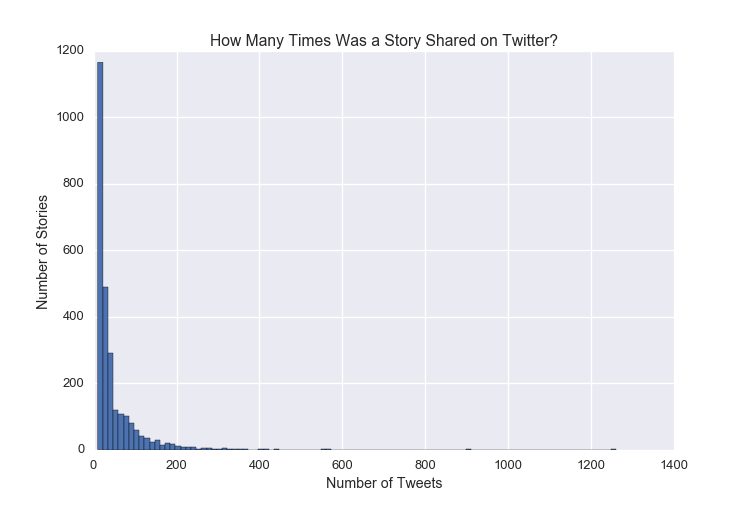
\includegraphics[width=0.8\textwidth]{story-share-dist}  
  \caption{Distribution of Story Shares
    \label{fig:story-share-dist}}
\end{figure} 

Story sharing behavior follows an approximate power law distribution. On average, stories are shared 46 times, however, the median (50th percentile) of shares is just 26. 


CNN, Politico, and Fox lead in publication popularity with the highest number of stories shared by tweets in our dataset-- likely due to the volume and close association to political content of the companies. Because our data pipeline detailed in the previous chapter looks for election-related news, outlets which track the campaign extensively are more likely to show up in our results.


\begin{figure}[H]  
\centering 
  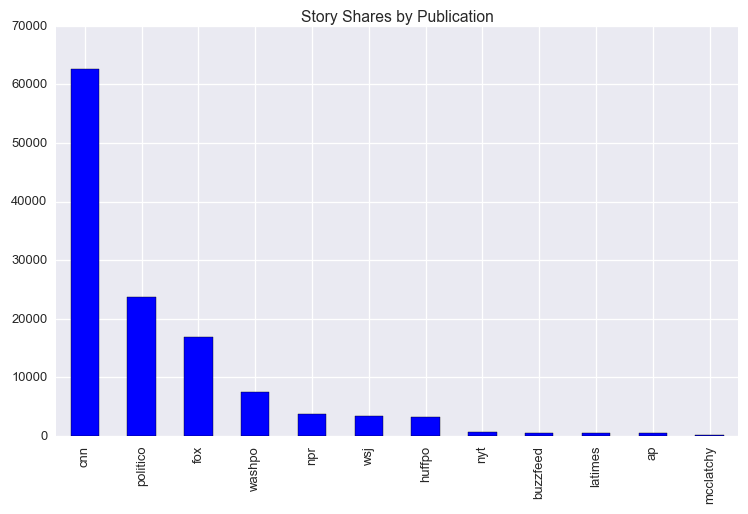
\includegraphics[width=0.8\textwidth]{all-stories-by-pub}  
  \caption{Number of story shares by publication
    \label{fig:tweets-by-pub}}
\end{figure} 


\newpage %force table to get on the next page

Examining the top 10 most shared stories, it comes as no surprise that outsized personality Donald Trump is by far the most ``tweetable'' candidate, dominating the list with 7 out of 10 stories featuring his name in the title.

 
\begin{table}
%\begin{tabular}{| l || c |} 
\begin{tabular}{ |l c| } 
    %s\toprule
    \hline
    Article &  \# tweets \\
    \hline
    %\midrule
    The One Weird Trait That Predicts Whether You're a Trump Supporter &   1260 \\
    Donald Trump Is Shocking, Vulgar and Right                         &    901 \\
    Biden praises Sanders on income inequality                         &    563 \\
    Why I'm voting for Trump                                           &    554 \\
    Anne Frank's stepsister compares Donald Trump to Adolf Hitler      &    445 \\
    Trump basks in his spotlight                                       &    436 \\
    Rubio: Law-abiding undocumented immigrants could stay              &    413 \\
    Terrorists use Trump's `Muslim ban' speech in recruitment video    &    398 \\
    Iowa caucuses: Donald Trump's moment of truth                      &    364 \\
    GOP senators: If Cruz wins, we lose                                &    357 \\
    %\bottomrule
    \hline
\end{tabular}
\caption{\label{tab:top-10}Top 10 Shared Stories}
\end{table}

The \emph{extent} to which he is prominent in articles is clear: by coding each story by the most frequently mentioned candidate, Trump has nearly three times as much coverage at nearly 60\% as the runner-ups, Ted Cruz and Hillary Clinton.

The large number of stories with Cruz as the most-mentioned candidate are likely due to his association to Trump as a Republican runner-up: 96\% of stories where Cruz is the most-mentioned candidate feature Trump as the second-most frequently occuring.

\begin{figure}[H]  
\centering 
  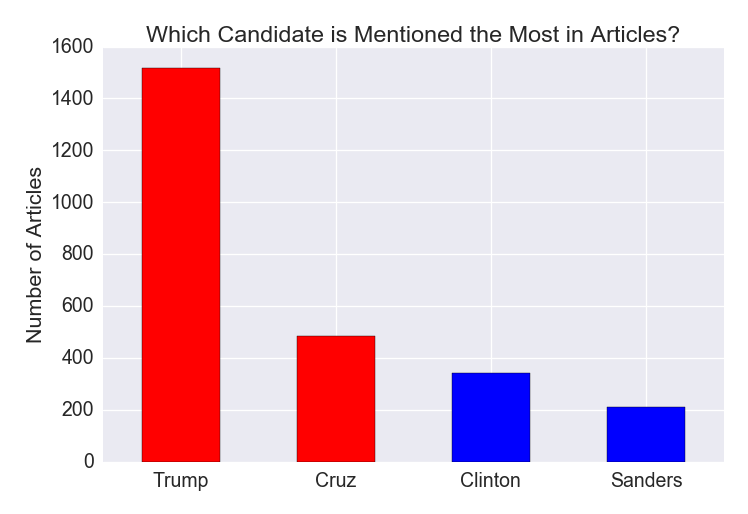
\includegraphics[width=0.8\textwidth]{candidate-mentions}  
  \caption{Number of story shares by publication
    \label{fig:tweets-by-pub}}
\end{figure} 




%% Same table but include Publication

% \begin{table}
% %\begin{tabular}{| l || c |} 
% \begin{tabular}{ |l c c| } 
%     \hline
                                                            
%     Article & Publication &   \# tweets    \\
%     GOP senators: If Cruz wins, we lose & cnn &   357 \\
%     Iowa caucuses: Donald Trump's moment of truth &  cnn   &   364 \\
%     Terrorists use Trump's `Muslim ban' speech in recruitment video &   cnn  &   398 \\
%     Rubio: Law-abiding undocumented immigrants could stay & politico &   413 \\
%     Trump basks in his spotlight & cnn &   436 \\
%     Anne Frank's stepsister compares Donald Trump to Adolf Hitler &  cnn   &   445 \\
%     Why I'm voting for Trump &  cnn   &   554 \\
%     Biden praises Sanders on income inequality &   cnn  &   563 \\
%     Donald Trump Is Shocking, Vulgar and Right & politico &   901 \\
%     The One Weird Trait That Predicts Whether You’re a Trump Supporter &  cnn   &  1260 \\
%     \hline
% \end{tabular}
% \caption{\label{tab:top-10}Top 10 Shared Stories}
% \end{table}


 















  
 


% \section{Tweets}

% \begin{figure}[H]  
% \centering 
%   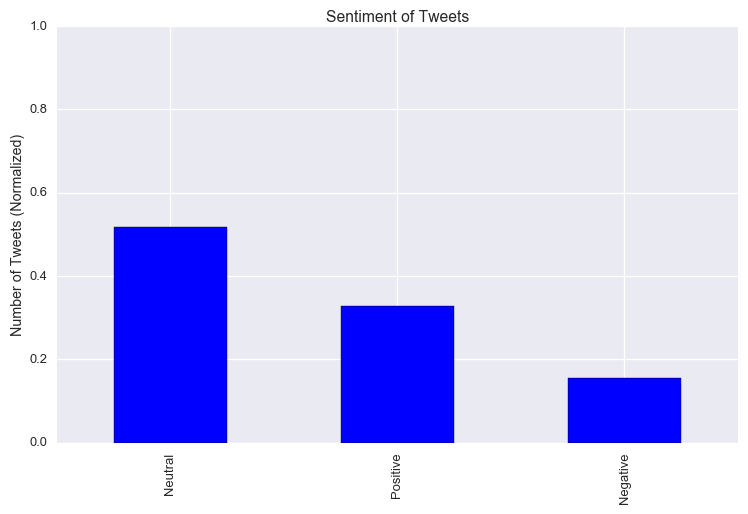
\includegraphics[width=0.9\textwidth]{all-tweets-sentiment}  
%   \caption{Sentiment of Tweets
%     \label{fig:data-stack-Twitter}}
% \end{figure} 


% \section{Tweeters}


%  \subsection{Descriptives}
%  \subsection{Story Length}
%  \subsection{Emotionality}
%  \subsection{Positivity}

%   \section{By Candidate}
%  \subsection{Descriptives}
%  \subsection{Story Length}
%  \subsection{Emotionality}
%  \subsection{Positivity}


%   \section{By Degree of Political Engagement}
%  \subsection{Descriptives}
%  \subsection{Story Length}
%  \subsection{Emotionality}
%  \subsection{Positivity}

%  \section{Trust and Virality? Test}